\documentclass[11pt]{article}
\usepackage{fullpage}
\usepackage{graphicx}
\usepackage{tikz}
\usepackage{hyperref}

\title{CS63 Fall 2022\\Lab 5: Explaining XOR Network}
\author{Yael N Borger, Delaney Hawkins}

\begin{document}

\maketitle

With random seed 11
the XOR network achieved 100\% accuracy on the XOR data set after
\ 1,109 %TODO: replace ldots with epochs
training epochs (we set for 25000, this was a nice surprise).  The resulting neural network is shown in the
following diagram.

%TODO: fill in the weights with ONE DECIMAL DIGIT of precision
\begin{center}
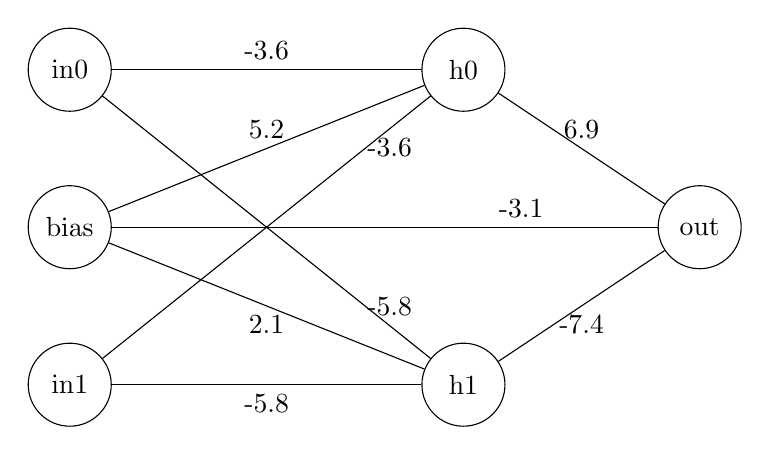
\begin{tikzpicture}
\tikzstyle{neuron}=[draw, circle, minimum size=30pt]

\draw (0,2) node[neuron] (bias) {bias};
\draw (0,4) node[neuron] (in0) {in0};
\draw (0,0) node[neuron] (in1) {in1};
\draw (5,4) node[neuron] (h0) {h0};
\draw (5,0) node[neuron] (h1) {h1};
\draw (8,2) node[neuron] (out) {out};

\draw (in0) edge node[above] {-3.6} (h0);
\draw (in0) edge node[very near end, above] {-5.8} (h1);
\draw (in1) edge node[very near end, below] {-3.6} (h0);
\draw (in1) edge node[below] {-5.8} (h1);
\draw (h0) edge node[above] {6.9} (out);
\draw (h1) edge node[below] {-7.4} (out);
\draw (bias) edge node[above] {5.2} (h0);
\draw (bias) edge node[below] {2.1} (h1);
\draw (bias) edge node[near end, above] {-3.1} (out);
\end{tikzpicture}
\end{center}

Based on these weights, this network solves XOR as follows.

% TODO: Explain how the network solved the XOR problem based on these
% parameters.
%oops, neither of us use latex! we fixed the enter spaces! :P
Our Network solved the XOR problem by receiving the inputs given and, using the weights, calculating the outputs. The weight multiplied by the inputs would result in a number that would be added to the other numbers that were being sent into another layer, and that resulting sum would be compared to a 0 (if it is greater than 0, the group would send forward a 1 and consider the node active, if it was 0 or below the group would send a 0 to the next node). These are the calculations our Network would be using that would make XOR work:

0,1 \newline
in0 = 0 \newline
in1 = 1 \newline
h0 = in0(-3.6) = 0 \newline
    +bias(5.2) = 5.2 \newline
    +in1(-3.6) = -3.6 \newline
    = 1 (active)\newline
h1 = in0(-5.8) = 0 \newline
    +bias(2.1) = 2.1 \newline
    +in1(-5.8) = -5.8 \newline
    =  0 \newline
out = h0(6.9) = 6.9 \newline
    +bias(-3.1) = -3.1 \newline
    +h1(-7.4) = 0 \newline
    = 1 (active) \newline

1,0 \newline
h0 = in0(-3.6) = -3.6 \newline
    +bias(5.2) = 5.2 \newline
    +in1(-3.6) = 0 \newline
    = 1 (active)\newline
h1 = in0(-5.8) = -5.8 \newline
    +bias(2.1) = 2.1 \newline
    +in1(-5.8) = 0 \newline
    = 0 \newline
out = h0(6.9) = 6.9 \newline
    +bias(-3.1) = -3.1 \newline
    +h1(-7.4) = 0 \newline
    = 1 (active)\newline

1,1 \newline
h0 = in0(-3.6) = -3.6 \newline
    +bias(5.2) = 5.2 \newline
    +in1(-3.6) = -3.6 \newline
    = 0\newline
h1 = in0(-5.8) = -5.8 \newline
    +bias(2.1) = 2.1 \newline
    +in1(-5.8) = -5.8 \newline
    = 0 \newline
out = h0(6.9) = 0 \newline
    +bias(-3.1) = -3.1 \newline
    +h1(-7.4) = 0 \newline
    = 0 \newline
    
0,0\newline
h0 = in0(-3.6) = 0 \newline
    +bias(5.2) = 5.2 \newline
    +in1(-3.6) = 0 \newline
    = 1 (active)\newline
h1 = in0(-5.8) = 0 \newline
    +bias(2.1) = 2.1 \newline
    +in1(-5.8) = 0 \newline
    = 1 (active)\newline
out = h0(6.9) = 6.9 \newline
    +bias(-3.1) = -3.1 \newline
    +h1(-7.4) = -7.4 \newline
    = 0 \newline 
    
\end{document}
